\chapter[Background]{Background}

This thesis is built up using many backgrounds on memory management, the
Windows internals and some malware prevention technology. This chapter will
give readers a quick summary to understand these key points. The chapter
heavily depends on these materials \cite{ligh2014art}
\cite{russinovich2012windows}.

\section[Fundamental OS]{Fundamental OS}

Understanding how the operating system works is fundamental when developing a
forensics tools. In this thesis, the OS memory management is a required
knowledge. Which is why in this section, we will go through these OS concepts,
pagination, virtual memory, and the OS kernel.

\subsection[Pagination]{Pagination}

Pagination, or paging, is a memory management scheme used by many modern
operating systems. In this scheme, the operating system handles memory by
blocks of constant size. A block of constant size is called a \textit{page}.
The operating system considers a process as a list of pages when using pagination,
and the physical memory RAM (random-access-memory) as a page holder. When
starting a process, the OS will not load the whole process in RAM but only
loads pages that need to be run. When a page in RAM is no longer needed, it
will be removed, \textit{page out}, and replaced by a higher priority page.
The convention \textit{in memory} states that the page is inside RAM, and a
page not inside RAM is said to be \textit{is disk}. In Figure
\ref{fig:pagination} we can see the OS loads some pages of the process in
memory, and the other pages are in disk.

\begin{figure}[h]
  \centering
  \caption{Pagination}
  \label{fig:pagination}
  \includegraphics[scale=0.7]{images/pagination.png}
\end{figure}

\subsection[Virtual memory]{Virtual memory}

Virtual memory is a memory management technique where the OS gives an
abstraction level over the addresses indexable by a process. The OS creates a
different address mapping schema for every process running; in other words, two
processes both access the same address results in a different address in RAM.
It is illustrated in Figure \ref{fig:virtualmem}, the two processes have the
same referencing address 0x4000, but in RAM, their addresses are 0x6000 and
0x9000. The address before conversion to RAM address is called virtual address,
and the RAM address is called physical address.

\begin{figure}[h]
  \centering
  \caption{Virtual memory}
  \label{fig:virtualmem}
  \includegraphics[scale=0.8]{images/virtualmem.png}
\end{figure}

\subsection[Kernel]{Kernel}

The kernel in OS is the program responsible for communicating with the hardware
and controlling other programs. The code for the kernel is loaded in memory
during the machine uptime. The kernel manages critical tasks, including
processes scheduling, memory management, I/O operations.

The kernel handles communication with the hardware through system calls or
\textit{syscall}. There are many implementations to the system call, and the
most common way is by system interrupts.  The kernel will have a syscall table,
which is a table of function pointers. They are called by an interrupt
instruction with the index to the syscall table, as shown in Figure
\ref{fig:syscall}.

\begin{figure}[h]
  \centering
  \caption{System call}
  \label{fig:syscall}
  \includegraphics[scale=0.7]{images/syscall.png}
\end{figure}

\subsection[Windows implementation]{Windows implementation}

In Windows 64-bit, pagination is implemented using pages of size 4KB.  Paged
out pages are saved in \texttt{C:\textbackslash\textbackslash Pagefile.sys}.
Virtual memory for every user processes is from 0x0000000000 to 0x7FFFFFFFFFF.
The address from 0x80000000000 to 0xFFFFFFFFFFF is called the system address
space or kernel space.  The system address space is only accessible by the
processes in \textit{kernel-mode}, namely the kernel and kernel drivers.  For
each user process, a separate address space is assigned for the process, but
there is only one system address space and is shared with every kernel
processes running. The user address space and the system address space are
virtual memory, which has to be translated to physical address when access. The
Figure \ref{fig:winimplement} shows the memory layout of the kernel and user
processes memory in Windows 64-bit systems. While the user process can not
access system address space, kernel processes can access any virtual page.

\begin{figure}[h]
  \centering
  \caption{Windows memory layout}
  \label{fig:winimplement}
  \includegraphics[scale=0.7]{images/winimplement.png}
\end{figure}

Syscall in Windows is called in two ways, and both implemented with a system
call table. The first way is done by interrupting the code 0x2e, and the second
way is using the instruction sysenter/syscall. Both ways receive the index to
the system call table in register edx.

\section[Windows Internal]{Windows Internal}

In this section, we introduce some key points of the Windows operating system.
These key points are executive objects, the kernel pool, the global list, and
debug symbols used by Windows.

\subsection[Executive Objects]{Executive Objects}

Windows executive objects are kernel structures allocated and prepended with
various headers. Only some kernel structures are allocated this way, a common
list of executive objects often used for forensics is in the Table
\ref{tab:execobj}. Executive objects must have a header called
\texttt{\_OBJECT\_HEADER}, but it can have other optional headers data.
Forensics tools often use these headers' data to get some general information
about the allocation. Below we discuss some kernel structures and their roles
in the Windows operating system.

\begin{table}[t]
\centering
\begin{tabular}{ll}
\hline
  Object        & Structure                         \\ \hline
  Process       & \texttt{\_EPROCESS}               \\
  Thread        & \texttt{\_ETHREAD}                \\
  File          & \texttt{\_FILE\_OBJECT}           \\
  Driver        & \texttt{\_DRIVER\_OBJECT}         \\
  Mutex         & \texttt{\_KMUTANT}                \\
  Token         & \texttt{\_TOKEN}                  \\
  Symbolic link & \texttt{\_OBJECT\_SYMBOLIC\_LINK} \\
  Type          & \texttt{\_OBJECT\_TYPE}           \\
  Key           & \texttt{\_CM\_HIVE}               \\
\end{tabular}
\caption{Comprehensive list of executive objects}
\label{tab:execobj}
\end{table}

\subsubsection[EPROCESS]{EPROCESS}

\texttt{\_EPROCESS}, Listing \ref{lst:eprocess}, is a structure to manage the
running process. This structure contains the process id, the parent process id,
the memory map for the process, the process environment block, the pointer to
list of loaded modules, the pointer to list of threads created by the process
and other information related to the process.  This structure is also a node in
a circular doubly linked list of processes.

The memory map is the list of sections inside a process address space, and
these are code, data, heap, libraries. It is represented as a self-balancing
tree where each node contains the address, size, and operations
(Read/Write/Execution) allowed in the region. This tree is often called as
\textit{Vad tree}, and the root of the tree is the \texttt{VadRoot} member in
\texttt{\_EPROCESS}.

The process environment block (PEB), Listing \ref{lst:peb}, contains the
information to the process, such as the image base address, the heap pointer.
This block resides in the user space memory, so the kernel process can not read
this information without mapping the user space into the kernel space. The
pointer to the address of the block is the \texttt{PEB} member of
\texttt{\_EPROCESS} and we can map the page containing the PEB to read the
process information.

\begin{lstlisting}[language=windbg,lable={lst:eprocess},caption=\texttt{\_EPROCESS} in Windows 7,float,floatplacement=H]
kd> dt _EPROCESS
nt!_EPROCESS
   +0x168 CreateTime       : _LARGE_INTEGER
   +0x170 ExitTime         : _LARGE_INTEGER
   +0x180 UniqueProcessId  : Ptr64 Void
   +0x188 ActiveProcessLinks : _LIST_ENTRY
   +0x238 PhysicalVadRoot  : Ptr64 _MM_AVL_TABLE
   +0x258 Win32Process     : Ptr64 Void
   +0x290 InheritedFromUniqueProcessId : Ptr64 Void
   +0x2e0 ImageFileName    : [15] UChar
   +0x308 ThreadListHead   : _LIST_ENTRY
   +0x328 ActiveThreads    : Uint4B
   +0x338 Peb              : Ptr64 _PEB
   +0x448 VadRoot          : _MM_AVL_TABLE
\end{lstlisting}

\begin{lstlisting}[language=windbg,label={lst:peb},caption=\texttt{\_PEB} in Windows 7,float,floatplacement=H]
kd> dt _PEB
nt!_PEB
   +0x002 BeingDebugged    : UChar
   +0x003 ImageUsesLargePages : Pos 0, 1 Bit
   +0x003 IsProtectedProcess : Pos 1, 1 Bit
   +0x003 IsLegacyProcess  : Pos 2, 1 Bit
   +0x003 IsImageDynamicallyRelocated : Pos 3, 1 Bit
   +0x003 SkipPatchingUser32Forwarders : Pos 4, 1 Bit
   +0x008 Mutant           : Ptr64 Void
   +0x010 ImageBaseAddress : Ptr64 Void
   +0x018 Ldr              : Ptr64 _PEB_LDR_DATA
   +0x030 ProcessHeap      : Ptr64 Void
   +0x050 CrossProcessFlags : Uint4B
   +0x0c8 HeapSegmentReserve : Uint8B
   +0x0d0 HeapSegmentCommit : Uint8B
   +0x0d8 HeapDeCommitTotalFreeThreshold : Uint8B
   +0x0e0 HeapDeCommitFreeBlockThreshold : Uint8B
   +0x0e8 NumberOfHeaps    : Uint4B
   +0x0ec MaximumNumberOfHeaps : Uint4B
   +0x0f0 ProcessHeaps     : Ptr64 Ptr64 Void
\end{lstlisting}

\subsubsection[ETHREAD]{ETHREAD}

\texttt{\_ETHREAD}, Listing \ref{lst:ethread}, is a structure used to manage
threads. This structure contains the process id, the thread id, the pointer to
the owner \texttt{\_EPROCESS}, the current thread state, threads flags. This
structure is also a node in a circular doubly linked list of threads. The
status of the thread can tell whether the thread is initilized, ready, running,
or waiting.  The thread waiting reason can also be found in this structure.
Thread's flags indicate the thread to be terminated, dead, hided from debugger,
impersonating, a system thread.

\begin{lstlisting}[language=windbg,label={lst:ethread},caption=\texttt{\_ETHREAD} in Windows 7,float,floatplacement=H]
kd> dt _ETHREAD
nt!_ETHREAD
   +0x000 Tcb              : _KTHREAD
      +0x164 State            : UChar
      +0x210 Process          : Ptr64 _KPROCESS or _EPROCESS
      +0x26b WaitReason       : UChar
   +0x360 CreateTime       : _LARGE_INTEGER
   +0x368 ExitTime         : _LARGE_INTEGER
   +0x378 ExitStatus       : Int4B
   +0x388 StartAddress     : Ptr64 Void
   +0x3b0 Cid              : _CLIENT_ID
      +0x000 UniqueProcess    : Ptr64 Void
      +0x008 UniqueThread     : Ptr64 Void
   +0x420 ThreadListEntry  : _LIST_ENTRY
   +0x448 CrossThreadFlags : Uint4B
\end{lstlisting}

\subsubsection[KMUTANT]{KMUTANT}

\textit{Mutant} is the way Windows name \textit{mutex}, a lock to prevent
multiple threads accessing the same time, and represented using a
\texttt{\_KMUTANT}, Listing \ref{lst:kmutant}.  \texttt{\_KMUTANT} has a
pointer to the thread owning the mutant.

\begin{lstlisting}[language=windbg,label={lst:kmutant},caption=\texttt{\_KMUTANT} in Windows 7,float,floatplacement=H]
kd> dt _KMUTANT
nt!_KMUTANT
   +0x018 MutantListEntry  : _LIST_ENTRY
   +0x028 OwnerThread      : Ptr64 _KTHREAD
\end{lstlisting}

\subsubsection[DRIVER\_OBJECT]{DRIVER\_OBJECT}

Every driver loaded and running will be represented with a type of
\texttt{\_DRIVER\_OBJECT}, Listing \ref{lst:driverobj}.  This structure
contains a pointer to the underlying device and functions related to this
driver. Functions related to the driver are \textit{init}, \textit{unload} and
28 major functions. 28 major functions are functions for interacting with the
system. These functions by default point to the kernel functions, but the
driver can register these function to the desired function. E.g, the fourth
function \texttt{IRP\_MJ\_READ} will be called when the user application calls
\texttt{ReadFile} or a kernel-mode driver calls \texttt{ZwReadFile}, by default
it is pointed to a routine which indicate \textit{not supported}, but the
driver can overwrite this to the desired function, as in Listing
\ref{lst:majorfunc}.

\begin{lstlisting}[language=windbg,label={lst:driverobj},caption=\texttt{\_DRIVER\_OBJECT} in Windows 7,float,floatplacement=H]
kd> dt _DRIVER_OBJECT
nt!_DRIVER_OBJECT
   +0x000 Type             : Int2B
   +0x002 Size             : Int2B
   +0x008 DeviceObject     : Ptr64 _DEVICE_OBJECT
   +0x018 DriverStart      : Ptr64 Void
   +0x020 DriverSize       : Uint4B
   +0x028 DriverSection    : Ptr64 Void
   +0x030 DriverExtension  : Ptr64 _DRIVER_EXTENSION
   +0x038 DriverName       : _UNICODE_STRING
   +0x048 HardwareDatabase : Ptr64 _UNICODE_STRING
   +0x050 FastIoDispatch   : Ptr64 _FAST_IO_DISPATCH
   +0x058 DriverInit       : Ptr64     long
   +0x060 DriverStartIo    : Ptr64     void
   +0x068 DriverUnload     : Ptr64     void
   +0x070 MajorFunction    : [28] Ptr64     long
\end{lstlisting}

\begin{lstlisting}[language=cpp,label={lst:majorfunc},caption=\texttt{Seting MajorFunction} in kernel-mode driver,float,floatplacement=H]
void MyReadFunction(PDEVICE_OBJECT DriverObject, PIRP Irp) {
}

void DriverEntry(PDEVICE_OBJECT DriverObject, PUNICODE_STRING /* RegistryPath */) {
  DriverObject->MajorFunction[IRP_MJ_READ] = MyReadFunction;
}
\end{lstlisting}

\subsection[Other kernel structures]{Other kernel structures}

\subsubsection[LDR\_DATA\_TABLE\_ENTRY]{LDR\_DATA\_TABLE\_ENTRY}

Windows tracks \textit{modules}, dynamically loaded library, loaded in each
process by a structure called \texttt{\_LDR\_DATA\_TABLE\_ENTRY}, Listing
\ref{lst:ldr}, this structure is a node in three different circular linked
lists, \textit{in load} list, \textit{in memory} list, and \textit{in
  initilization} list. This structure contains the module's base address, the
pointer to the module's entry function, the module size, the module's name, and
the number of processes loaded this module. The kernel module is tracked using
\texttt{\_KLDR\_DATA\_TABLE\_ENTRY}, which has some small differences, but the
layout is almost the same. \texttt{\_KLDR\_DATA\_TABLE\_ENTRY} definition is
not publicly provided until Windows 10.

\begin{lstlisting}[language=windbg,label={lst:ldr},caption=\texttt{\_LDR\_DATA\_TABLE\_ENTRY} in Windows 7,float,floatplacement=H]
kd> dt _LDR_DATA_TABLE_ENTRY
nt!_LDR_DATA_TABLE_ENTRY
   +0x000 InLoadOrderLinks : _LIST_ENTRY
   +0x010 InMemoryOrderLinks : _LIST_ENTRY
   +0x020 InInitializationOrderLinks : _LIST_ENTRY
   +0x030 DllBase          : Ptr64 Void
   +0x038 EntryPoint       : Ptr64 Void
   +0x040 SizeOfImage      : Uint4B
   +0x048 FullDllName      : _UNICODE_STRING
   +0x058 BaseDllName      : _UNICODE_STRING
   +0x06c LoadCount        : Uint2B
\end{lstlisting}

\subsection[Kernel pool]{Kernel pool}
\label{sec:pool}

The kernel pool is the way Windows named the kernel heap for dynamic memory
allocation. There are many pools, each with different types, and the system
memory space has specific ranges for these pools. However, there are two main
types of pool, the \textit{paged pool}, and \textit{non-paged pool}. The paged
pool can be paged out to disk while the non-paged pool is always in memory for
every valid page. The non-paged pool is mostly used to allocate system
structures because they must always be in memory for critical access.  We call
the allocation inside a pool a \textbf{block}. A block has a header of type
\texttt{\_POOL\_HEADER} and the data. The pool header contains the size of the
allocation, the size of the previous allocation, the type of the pool
allocated, and a four-byte tag. The size in the header is a multiplier of 16 in
64-bit systems.  The type of pool is an enumeration, and it should match the
pool type where the block was allocated.  The four-byte tag is a value provided
when allocate the block using legacy Windows API such as
\texttt{ExAllocatePoolWithTag}. In Figure \ref{fig:pooltag}, we can see how the
pool allocation works.

\begin{figure}[h]
  \centering
  \caption{Pool Allocation}
  \label{fig:pooltag}
  \includegraphics[scale=0.7]{images/pooltag.png}
\end{figure}

The pool that is relevant to the kernel data is called the non-paged pool. This
pool's pages are never paged out to disk and contain many kernel objects.  The
header of blocks allocated inside this pool will have the type value equal to
2. Kernel objects are allocated inside this pool with a tag hard-coded inside
the Windows source-code. Their tags and the structure are described in the
Table \ref{tab:pooltag}.

\begin{lstlisting}[language=windbg,caption=\texttt{\_POOL\_HEADER} in Windows 64-bit,float,floatplacement=H]
kd> dt _POOL_HEADER
nt!_POOL_HEADER
   +0x000 PreviousSize     : Pos 0, 8 Bits
   +0x000 PoolIndex        : Pos 8, 8 Bits
   +0x000 BlockSize        : Pos 16, 8 Bits
   +0x000 PoolType         : Pos 24, 8 Bits
   +0x004 PoolTag          : Uint4B
\end{lstlisting}

\subsection[Global list]{Global list}

Windows has several global lists to control the systems, the head (pointer) of
these lists is saved inside global variables in the kernel. For processes,
Windows has two circular doubly linked lists, indexed by
\texttt{PsActiveProcessHead}, \texttt{KiProcessListHead}.  There is also a
handle table list, \texttt{HandleTableListHead}, where each handle has a
pointer to \texttt{\_EPROCESS}. Kernel modules are also stored inside the
\texttt{PsLoadedModuleList}.

\subsection[Debug symbols]{Debug symbols}

The Windows source code is not publicly available, however Windows distributes
debug symbols for researching purposes. These debug symbols contains the offset
to global variables, functions and structures layout. The symbols are compressed
into a file called program database, or \textit{PDB}, with the extension
\texttt{.pdb}. The instruction to extract the file is limited described
\cite{microsoft-pdb}, but public works have been done and parsers are
available.

A PDB file is unique to one specific version of a kernel module. The PDB file
for the main kernel module is named \texttt{ntkrnlmp.pdb} for the kernel module
\texttt{C:\textbackslash \textbackslash Windows \textbackslash System32
\textbackslash ntoskrnl.exe}. The binary \texttt{ntoskrnl.exe} is different
across Windows updates. Downloading a specific PDB file for the kernel requires
the module's id, \textit{GUID}, and \textit{age}. GUID and age are parsed from
the binary in the RSDS section of a PE file \footnote{Executable file in
Windows OS}. In the same Windows version, specifically the Windows minor
version, structures layout are the same, but addresses to global variables and
functions are different.  Across different Windows' major version, huge changes
in structure layout, new functions and variables were introduced, and old ones
were removed. This is why downloading the correct PDB file for the current
machine is better than hardcoding the addresses, and members offset.

The Microsoft PDB server hosting the PDB files is located at
\url{https://msdl.microsoft.com/download/symbols}. To download the main kernel
module, we need to build the request URL as defined in Listing
\ref{lst:downloadpdb}. After that, parsing the PDB can be done using public
libraries, PDB parser by Brendan\cite{pdbparse} or PDB by Will
Glynn\cite{pdbrust}.

\begin{lstlisting}[language=cpp,caption=Download PDB file,label={lst:downloadpdb},float,floatplacement=H]
const string root_url = "https://msdl.microsoft.com/download/symbols/";
const string pdb_name = "ntkrnlmp.pdb";
const string guid = "XXXX";
const string age = "01";

const string download_url = root_url + pdb_name + "/"
                          + guid + age + "/"
                          + pdb_name;
\end{lstlisting}

\section[Prevention]{Prevention}

To prevent malware infiltration, both the Windows development team and
Anti-Virus vendors have tried to apply new technology to secure the operating
system. Here we list some advancement that has helped minimize the spread of
malware.

\subsection[Signature enforcement]{Signature enforcement}

In the past, drivers can be loaded on the system with only an admin privilege.
It was a bad practice, any driver, trusted or untrusted, can be loaded inside
Windows. Windows then forces driver creators/distributors to sign their drivers
using a Windows certificate to prevent untrusted drivers. Signing the driver
costs money and includes a code review that would prevent a malicious driver
created.

However, some malware writers are brilliant, they could reuse a legitimate
driver with vulnerability and \textit{exploit} the driver to make it work as
they wanted. The driver is trusted, but the bug inside the driver is used as an
attack vector. An example is RobinHood (2020) malware reused the
\texttt{GDRV.SYS} driver from Gigabyte \cite{robinhood}.

\subsection[Patchguard]{Patchguard}

Windows prevents malware from modifying kernel components with Patchguard.  In
the past, malware used to \textit{patch}, modify, some kernel components to
gain control of the system.  It was prevented after Windows introduced
Patchguard, a way to detect edits in the kernel code and crash the system when
editing detected.

Although this was a good approach, Windows still has some failure. The report
on malware bypassing Patchguard is GhostHook (2017) \cite{ghosthook}, and two
research to bypass the Patchguard are InfinityHook (2019) \cite{infinityhook},
and ByePg (2019) \cite{byepg}.

\subsection[On-access scanning]{On-access scanning}

On-access scanning is a technique developed by Anti-Virus vendors to scan the
file for malware evidence on accessing the file. They installed a hook in the
Windows API for file access, and scan the file on any read/write access. If the
file matches a previously defined signature, the Anti-Virus will prevent access
and warn the user for removal. The algorithm is illustrated in Figure
\ref{fig:onaccessscan}, this algorithm is used by McAfee Anti-Virus
\cite{onaccessscan}.

\begin{figure}[h]
  \centering
  \caption{McAffee On-access scanning}
  \label{fig:onaccessscan}
  \includegraphics[scale=0.8]{images/onaccessscan.png}
\end{figure}

Because the scan depends on the pre-defined signature, a new malware could
bypass these rules if it uses a novel method to infect or hide. The rules can
be bypassed by applying obfuscation in the malware code, which hides traces of
evident behavior.

Scanning for signature using machine learning is still a new method, and even
though some vendors tried, the progress is not much positive. A security
researcher has created a sample malware bypassing the Cylance Smart Anti-Virus
in less than 15 minutes \cite{cylance}.


\chapter[Hidden malware and memory forensics]{Hidden malware and memory forensics}

Malware has many ways to run inside the system. It can create a process, create
a thread, load a library, or run a driver. A hidden malware will make these
objects can not be found when using Windows API or by traversing the legacy
lists.  For example, there are Windows APIs that can get information on
processes, threads, libraries, drivers, \texttt{EnumProcesses},
\texttt{Thread32First}, \texttt{EnumDeviceDrivers},
\texttt{NtQuerySystemInformation}. Malware will try to remove itself from these
API results. Thus, if an inspection system uses these API, the malware present
is not shown. To reveal the malware, one has to use forensics methods,
including but not limited to memory forensics.  In this chapter, we present in
technical terms how malware interfere with the system in order to hide and how
forensics investigators can find them using memory forensics.

\section[Process hiding]{Process hiding and rootkits}

In this section, we review the techniques used by malware to hide themselves
both on user space and kernel space. Most malware tries to infiltrate the
kernel space because it gives them more power to the system. These types of
malware running in kernel space are often referred to as rootkits. Rootkits are
hard to detect because they often hide from global lists.

\subsection[SSDT hooking]{SSDT hooking}

SSDT, short for System Service Descriptor Table, is a system call table in
Windows. SSDT hooking is the way malware rewrite the table and edit some
entries to the malware's function. A better way of rewriting is editing the
function into jumping or calling the malware's function. Of course, the malware
function must somehow perform the system function so that the OS can still be
running. In Figure \ref{fig:ssdt}, we show how SSDT hooking is done. The figure
shows a function in the SSDT is hooked and pointed to a function inside
\texttt{malicious.dll}.

\begin{figure}[h]
  \centering
  \caption{SSDT hooking}
  \label{fig:ssdt}
  \includegraphics[scale=1]{images/ssdt.png}
\end{figure}

On p32-bit systems, each thread has a different SSDT, which can be edited (by
kernel process). Because this table is only visible to one thread, the malware
can modify it without changing the system table.

SSDT hooking is stealth and dangerous. A hooked SSDT function can alter the
result returned to hide the malware. As bad as it could be, many years ago
Anti-Virus software used this to monitor system calls
\cite{case2020hooktracer}. They track the calls to SSDT, e.g., the create file
system call and monitor what file is being created and apply some checks to see
if the action will harm the system, e.g., writes a malware to file.

\subsection[IRP hooking]{IRP hooking}

Each kernel driver has a list of 28 major functions used for communicating with
other processes, editing any of the 28 major functions is called IRP hooking.
IRP, \textit{I/O Request Packets}, is the data sent when the user application
communicates with the driver. IRP contains the index to the 28 major functions
to ask the driver to perform. A malware could change the major function list so
that the driver calls the malware's function.  IRP hooking is done either by
replacing the pointer or editing the function into jumping or calling the
malware's function. An advanced technique of IRP hooking, the malware allocates
a small section inside the driver and writes the malware's code then rewrites
the IRP functions into this code. Figure \ref{fig:irp} shows how IRP hooking is
done.

\begin{figure}[h]
  \centering
  \caption{IRP hooking}
  \label{fig:irp}
  \includegraphics[scale=0.5]{images/irp.png}
\end{figure}

\subsection[DKOM]{DKOM}

DKOM is short for Direct Kernel Object Manipulation. It is when a malware
rewrites the kernel object members. One of the most used tricks related to DKOM
is removing object(s) from the linked list of the object, as shown in Figure
\ref{fig:dkom}. The removed object is not freed, and continue running inside
the memory.

\begin{figure}[h]
  \centering
  \caption{DKOM remove a node from linked list}
  \label{fig:dkom}
  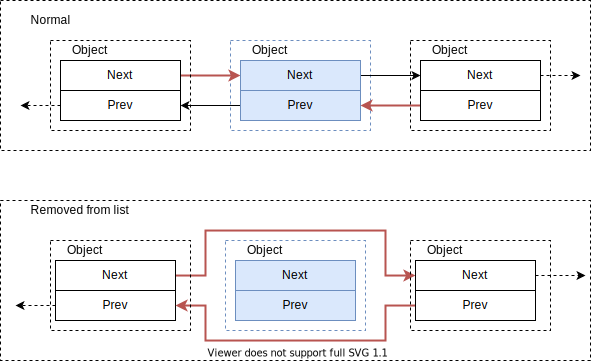
\includegraphics[scale=0.7]{images/dkom.png}
\end{figure}

The process list is a doubly-linked list, by removing the index to the desired
process malware can hide from windows API enumeration and list traversing.

The doubly-linked lists of loaded modules, namely \texttt{in load}, \texttt{in
memory}, \texttt{in initilization}, can all be edited to remove the module. A
naive malware will remove itself from the \texttt{in load} list, but a
comparison with the other two lists can reveal the hidden module. A better
hiding malware will try to remove itself from these three lists.

If the malware wants to hide one of its threads, it removes the thread from the
threads list, the pointer to the thread list is \texttt{ThreadListHead} in
\texttt{\_EPROCESS}.

Removing a node from the linked list is a common task, but DKOM is not limited
to these techniques, the malware can edit many members. An old
research\cite{robussignature} made by Brendan on Windows XP reveals that of the
72 selective members from selective structures, 29 members can be modified
without affecting, crashing, the system.  However, this research needs to be
updated with Windows 10. From the research results, malware can edit many
members, some of which will make them hidden from the system without breaking
the system.

\section[Memory Forensics]{Memory Forensics}

With all the preventions, malware still finds a way to bypass the security
setup and infect the system. When such an event occurs, a skilled technician
will begin analyzing the system. To start the investigation, they would need to
take the physical memory content of the system and analyze the content looking
for prominent malware. This is called memory forensics, a sophisticated process
done by a team of security researchers when a breach occurs or when an unknown
factor compromises the system.

\subsection[Memory acquisition]{Memory acquisition}

The first step in memory forensics is capturing the content of physical memory.
This step is often called as \textit{memory acquisition}. The goal was to load
the RAM data inside a file. There are multiple ways \cite{memoryAcquisition} to
do this in a running machine using a kernel driver:

\begin{enumerate}
\item Read \texttt{\textbackslash\textbackslash.\textbackslash PhysicalMemory}
\item Use \texttt{MmMapMemoryDumpMdl}
\item Use \texttt{MmMapIoSpace}
\item PTE remapping
\end{enumerate}

The RAM is a device, and Windows exposes the device as a file with the absolute
path \texttt{\textbackslash\textbackslash.\textbackslash PhysicalMemory}. By
reading this file, we are accessing the RAM itself. However, Windows prevented
reading this file. The second and third method maps physical page(s) to the
kernel space, the content is sent back to the user space to write out the file.
The fourth method is a technique described by Michael Cohen and Johannes
Stüttgen \cite{pteremap} to capture the memory using the PTE, page table entry.

Most memory acquisition tools are closed source, the one open-source memory
acquisition tool is WinPmem \cite{winpmem} and using the third and fourth
method to capture the RAM. WinPmem's author also encourages using the PTE
remapping method for better results. Other programs often used for memory
acquisition are \texttt{DumpIt} by Moonsol, \texttt{FTK Imager} by AccessData,
\texttt{Belkasoft RAM Capturer} by Belkasoft.

Hypervisor, VirtualBox or VMWare, can generate the memory file.  Although the
memory file format is different from each virtual machine implementation, the
documentation of the file format is available online.

The last way to acquire the memory content is through Windows debug mechanism.
Windows has an option to generate the memory file when the system crash, if
this option is on, Windows will produce the file at \texttt{C:\textbackslash
Windows\textbackslash MEMORY.DMP} on system crash. Windows also has multiple
option to the memory file, such as the \textit{full dump}, \textit{mini dump},
\textit{kernel dump}. These files are not officially documented by Windows and
intended to be used by Windows debugger, but researchers have reversed the file
format for forensics purposes \cite{mdmpfile} \cite{dmpfile}.

\subsection[KDBG]{KDBG}

KDBG is a Windows structure for debugging purposes, this structure contains
pointers to many kernel essential components, such as the list of processes.
Finding this structure in the memory file will give some insight into the
system.  This structure can be found using the four-byte ``KDBG'' in Windows
versions before 8. In Windows 8 and above, the structure is encoded and makes
it more challenging to find the structure. However, by brute-scanning and
brute-decoding \cite{kdbgEncoded}, one can still find the structure.

\subsection[Pool tag scanning]{Pool tag scanning}

As described in Section \ref{sec:pool}, each block has a pool header contains a
four-byte tag. By scanning for a specific tag value that the OS uses to
allocate for a kernel structure, we can search for all the object allocated,
and sometimes de-allocated but not overwritten. Each tag-block matches should
be further checked for validity, the pool body size (block size subtract the
pool header size) should be bigger than the object holding (if the object is an
executive object), or equal to the object.  Optional checks for pool type value
are done with objects usually allocated in one pool section.  E.g.,
\texttt{\_EPROCESS} is always allocated inside the non-paged pool section,
hence the pool type is 2. This technique is called \textit{Pool tag scanning}
\cite{pooltagscan}, and often done by a full search in the memory file. In
2016, Sylve, Joe T and Marziale, Vico and Richard III, Golden G
\cite{sylve2016pool} improved this technique by locating the range of the
non-paged pool region and scan only the pages that are valid. They named the
technique \textit{Pool tag quick scanning}.

The pool tag quick scanning research is conducted on Windows Vista and 8, we
extended the findings of these ranges on Windows XP, 7, 8, and 10 (all versions
from 2015 to 2020), with reference from the Rekall project. The result can be
found in Table \ref{tab:nonpaged}.

\begin{table}[]
\begin{tabular}{lll}
\hline
Windows version & Pool start                      & Pool end                      \\ \hline
XP              & \texttt{nt!MmNonPagedPoolStart} & \texttt{nt!MmNonPagedPoolEnd} \\
7, 8, 8.1       & \texttt{nt!MiNonPagedPoolStart} & \texttt{nt!MiNonPagedPoolEnd} \\
10 2015         & \texttt{nt!MiState}
                & \texttt{nt!MiState} \\
                & \texttt{->SystemNodeInformation}
                & \texttt{->SystemNodeInformation} \\
                & \texttt{.NonPagedPoolFirstVa}
                & \texttt{.NonPagedPoolLastVa} \\
10 2016-2019    & \texttt{nt!MiState}
                & \texttt{nt!MiState} \\
                & \texttt{->Hardware}
                & \texttt{->Hardware} \\
                & \texttt{.SystemNodeInformation}
                & \texttt{.SystemNodeInformation} \\
                & \texttt{.NonPagedPoolFirstVa}
                & \texttt{.NonPagedPoolLastVa} \\
10 2020         & \texttt{nt!MiState}
                & \texttt{nt!MiState} \\
                & \texttt{->Hardware}
                & \texttt{->Hardware} \\
                & \texttt{.SystemNodeNonPagedPool}
                & \texttt{.SystemNodeNonPagedPool} \\
                & \texttt{.NonPagedPoolFirstVa}
                & \texttt{.NonPagedPoolLastVa} \\ \hline
\end{tabular}
  {\raggedright \texttt{nt!foo} is the address of \texttt{foo} in kernel space
    \par}
  {\raggedright \texttt{nt!MiState} is a pointer to the type
  \texttt{\_MI\_SYSTEM\_INFORMATION}, this structure layout is different with
  each Windows 10 releases \par}
  {\raggedright \texttt{nt!MiNonPagedPoolStart} or
  \texttt{nt!MiNonPagedPoolStartAligned} both valid for Windows 7, 8, 8.1. Aligned
  version points to the first valid page in the pool \par}

  \caption{Non paged pool start and end}
  \label{tab:nonpaged}
\end{table}

Pool tag scanning is often used to ensure there is no process hiding from the
kernel list by simple removal. Comparing the pool tag scanning result with the
list traversing, we may be able to reveal unlinked objects from the global
list. However, pool tag scanning can be used to reveal other objects often not
reside on any list. These can be internet-related structures, kernel callbacks.
Although Windows does not document this structure, many people have studied the
Windows source code (by reversing) and came up with structure definitions and
reasonable names. In Table \ref{tab:pooltag}, we list the tags and the
structure where pool tag scanning is often used to find. These tags are used in
the Volatility framework.

\begin{table}[]
\begin{tabular}{llll}
\hline
  Structure                 & Structure Name                     & Pool Tag (new) & Pool Tag (old)        \\ \hline
  Driver Object             & \texttt{\_DRIVER\_OBJECT}          & Driv           & Dri\textbackslash xf6 \\
  File Object               & \texttt{\_FILE\_OBJECT}            & File           & Fil\textbackslash xe5 \\
  Process                   & \texttt{\_EPROCESS}                & Proc           & Pro\textbackslash xe3 \\
  Thread                    & \texttt{\_ETHREAD}                 & Thre           & Thr\textbackslash xe5 \\
  Modules                   & \texttt{\_LDR\_DATA\_TABLE\_ENTRY} & MmLd           &                       \\
  TCP endpoint              & *\texttt{\_TCP\_ENDPOINT}          & TcpE           &                       \\
  TCP listener              & *\texttt{\_TCP\_LISTENER}          & TcpL           &                       \\
  UDP endpoint              & *\texttt{\_UDP\_ENDPOINT}          & UdpA           &                       \\
  TCP connection            & *\texttt{\_TCPT\_OBJECT}           & TCPT           &                       \\
  Notification Packet       & *\texttt{\_NOTIFICATION\_PACKET}   & IoFs           &                       \\
  Shutdown Packet           & *\texttt{\_SHUTDOWN\_PACKET}       & IoSh           &                       \\
  Generic callback          & *\texttt{\_GENERIC\_CALLBACK}      & Cbrb           &                       \\
  DbgPrint callback         & *\texttt{\_DBGPRINT\_CALLBACK}     & DbCb           &                       \\
  Registry callback         & *\texttt{\_REGISTRY\_CALLBACK}     & CMcb           &                       \\
  Hardware profile callback & *\texttt{\_NOTIFY\_ENTRY\_HEADER}  & Pnp9           &                       \\
  Device interface callback & *\texttt{\_NOTIFY\_ENTRY\_HEADER}  & PnpD           &                       \\
  Target device callback    & *\texttt{\_NOTIFY\_ENTRY\_HEADER}  & PnpC           &                       \\
\hline
\end{tabular}
  {\raggedright *: This structure is not documented by Windows, the name is taken
  from Volatility framework \par}
  \caption{Comprehensive list of pool tag and corespondent structure}
  \label{tab:pooltag}
\end{table}

\subsection[SSDT and IRP hook detection]{SSDT and IRP hook detection}

SSDT hooking is dangerous in a way it can modify the kernel system call
behavior.  Detection of SSDT involves finding the system table and locate the
function address between loaded modules.The SSDT is located at
\texttt{KiServiceTable}, with \texttt{KiServiceLimit} elements of 32-bit value.
Every element is an offset to the function of the SSDT. To retrieve the address
of the function, we follow Listing \ref{lst:ssdt}.


\begin{lstlisting}[language=cpp,caption={Retrieve SSDT functions},label={lst:ssdt},float,floatplacement=H]
int32_t* KiServiceTable;
int KiServiceLimit;
void* ssdt[KiServiceLimit];
for (int i = 0; i < KiServiceLimit; i++) {
  ssdt[i] = (void*) ((int64_t)KiServiceTable + (KiServiceTable[i] >> 4));
}
\end{lstlisting}

After recovering all the functions in the system call table, we will check
every loaded module of type \texttt{\_KLDR\_DATA\_TABLE\_ENTRY} and see if the
address of the function is in the range of the \texttt{DllBase} and
\texttt{DllBase + Size}, if the address is between this range, the function is
in this module.  Because these are system calls, the functions should reside in
the kernel module, \texttt{ntoskrnl.exe}. If some functions reside in another
module, the SSDT probably hooked. Some malware even modify the function
instruction to jump or call to itself, this can be check by dumping several
bytes at the function address and decompile into machine code checking for jump
instruction and check the referenced address module.

IRP hooking is in driver 28 major functions. To detect this type of hook, we
list the 28 major functions searching for the loaded modules containing these
functions. It should be noted that the driver should either have the IRP
functions belongs to the driver or the kernel modules. If the functions are of
another module, then it was probably hooked. If the malware patch the
underlying function to jump or call itself, decompile the first few bytes
looking for such instruction and check the referenced address' module. For
the advanced IRP hooking method, this can only be detected after reversing the
function being hooked.

% To make the result easier to read and understand, the loaded module are parsed
% to get the exported symbols. When printing out the result, the module name with
% the function name will be printed out.

\subsection[Unloaded kernel drivers]{Unloaded kernel drivers}

There are some cases where malware load and unload the kernel driver almost
immediately (Rustock). In these scenarios, looking inside the unloaded driver
list might shed some light on this type of malware. Windows stores a list of
unloaded kernel drivers, the pointer to the list is located at
\texttt{MmUnloadedDrivers}. The list contains at most 50 members sized 0x28
bytes, the first 0x18 bytes in each member is of type
\texttt{\_UNLOADED\_DRIVER}.  \texttt{\_UNLOADED\_DRIVER} only contains the
name of the driver and the start and end address of the driver, the
\texttt{\_DRIVER\_OBJECT}, in most cases, is deallocated. If lucky, pool tag
scanning may show drivers unloaded, but it is usually not the case.

